% !TEX root = main.tex
\section{Methodology}\label{sec:methodology}
In this section, we describe the methodology we use to characterize services hosted on anycast prefixes.

%\vspace{0.2em}\noindent\textbf{Service discovery measurements} --
%Furthermore, measurement tools have been developed to help identify services on a large scale~\cite{ZMapInternetScanner2013,lzr}.\rhl{can go to methodology}\todo[inline, inlinewidth=1cm, noinlinepar, size=\tiny]{G: moved}
%We perform measurements to characterize services on anycast prefixes.\verbose
While other service discovery data sets exist, \eg, \gls{cuids}~\cite{DurumericEtAl_CensysMapInternet_2025}, we opt to use our own scanning infrastructure. %\rhl{rephrase to state why Censys is not enough}\todo[inline, inlinewidth=2.5cm, noinlinepar, size=\tiny]{G: done}
%First, \laces covers short-term anycast prefixes (\ie, anycast for a single or few days) for which we require scanning data at daily granularity whereas \gls{cuids} provides weekly snapshots for researchers.
Due to the distributed nature of anycast, we investigate differences in service deployments amongst \glspl{pop} by probing from two \glspl{vp} on different continents.
Although \gls{cuids} is scanned from multiple \glspl{vp}~\cite{DurumericEtAl_CensysMapInternet_2025}, the \dataset does not provide information from \textit{which} \gls{vp} the results are from.
Furthermore, prior work indicates that network operators block \gls{cuids} scans more frequently than those originating from academic networks~\cite{wan-origin-scanning}.
Finally, we make all results collected using our scanning pipeline publicly available for reproducibility and future research~\cite{measurement-data}.

Our measurement pipeline scans both TCP and UDP ports.
For TCP, we detect open ports with ZMap~\cite{ZMapInternetScanner2013}, then we proceed with service detection using LZR~\cite{lzr} and ZGrab2~\cite{censys15}.
On UDP ports, we use ZMap's UDP probes and a QUIC probe~\cite{zirngibl2021over9000} to force QUIC version negotiation.
The TCP and UDP measurements are performed from two \glspl{vp}, one in Europe and one in Oceania.
The ZMap and LZR measurements are from February 18th, and the follow-up ZGrab2 measurement is from February 20th, 2026.
~\cref{fig:methodology} provides an overview of our pipeline. %\jz{Are the stages important? If so, can we make them visible in the figure? But I don't really see a value in them. The first stage is selecting the prefixes and the using a static config?}
% G: there is no importance on the stages. I divided to facilitate the explanation below. 

\begin{figure}[tb]
\centering
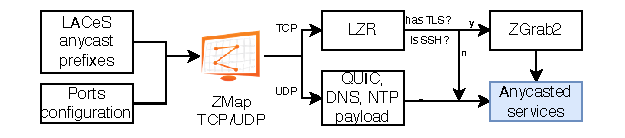
\includegraphics[width=\columnwidth]{./data/plots/measurement-pipeline.pdf}
\caption{Measurement pipeline overview. %\jz{After LZR, which path is yes or no to the question?} \jz{Why is ZGrab 1-off? What is the difference to LZR/ZMap then?} \jz{Unify capitalization in boxes.} %G: updated
}
%\vspace*{-4px}
\label{fig:methodology}
\end{figure}

As input, we retrieve anycast prefixes from \laces~\cite{Hendriks_LACeS_An_Open_2025}.
Whilst other anycast censuses exist,
we chose \laces because it provides an open-source \dataset that is extensively validated using ground truth.
%Additionally, it is the only census that provides geolocation of anycast prefixes, \ie, the anycast \glspl{pop}. \jz{Any source for this claim?} % G: I think this information is not even necessary to be mentioned.
On the TCP scans, we configure our scanning pipeline to use the 100 \texttt{nmap}'s most common ports~\cite{lyon2009nmap}, and we complement them with 18 additional ports associated with services that LZR supports. %\rhl{unclear. also: just opportunistic?}\todo[inline, inlinewidth=2.5cm, noinlinepar, size=\tiny]{G: clarified; additional ports to utilize the tool's capability}
On UDP, we scan the ports 53 (DNS, included in the \texttt{nmap}'s common ports), 123 (\gls{ntp}), 853 (\gls{doq}), and 443 (HTTP over QUIC).
Port 443 is an exception where we also scan on the TCP protocol. %\jz{Reviewer 2: This sums up to 121,  abstract says 120} %G: thanks! that's because the top 100 from nmap includes port 53.
%\rhl{We don't select each time we run the pipeline. Our selection is static.} G: removed UDP word, so now it doesn't confuse that we do dynamic port selection
%\jz{It still sounds like the selection of ports is dynamic as part of the pipeline} % G: changed the sentence.

We instrument LZR to follow the handshake order strategy proposed by Izhikevich \etal~\cite{lzr}.
%\rhl{I reworded, check}\todo[inline, inlinewidth=2.5cm, noinlinepar, size=\tiny]{G: ok}
Izhikevich \etal found that the most efficient initial step is to \textit{wait} for servers to send an initial packet, as certain protocols transmit a banner that can be fingerprinted upon connection (\eg, SSH, FTP, SMTP).
If no response is received from the server that can already be fingerprinted after the handshake, a protocol packet is sent.
For ports associated with one of LZR's 32 supported protocols, we structured our handshake sequence to begin with a \textit{wait} step, followed by the port's protocol-specific handshake, and subsequently a fallback sequence consisting of TLS, HTTP, DNS, and \gls{pptp} (as the sequence in~\cite{lzr}). % \jz{What is PPT? Introduce as acronym}. % G: my typo! it's pptp and added the acronym
This approach prioritizes detecting of expected services while robustly capturing anomalous applications running on standard ports.
For ports where LZR lacks specific service support, we directly applied the empirically derived handshake order proposed by Izhikevich \etal (Table 2 in~\cite{lzr}).
The authors demonstrated that this sequence of five handshakes successfully identifies over 99\% of unexpected services, allowing us to optimize our scanning efficiency without sacrificing detection coverage.
%\rhl{Evidence needed.}
%\rhtodo{The above needs a thorough revision.}
%\todo[inline, inlinewidth=2.5cm, noinlinepar, size=\tiny]{G: revised and added evidence.}
%See below limitations of our scanning strategy.\verbose

%For UDP scans, we use ZMap's UDP probes for DNS/53 and NTP/123 and we use a QUIC probe~\cite{zirngibl2021over9000} to force a QUIC version negotiation on ports 443 and 853.  % G: repetition; removed
We parse the DNS, \gls{ntp}, and QUIC responses using Python libraries for DNS~\cite{python-dns}, \gls{ntp}~\cite{python-ntp}, and QUIC~\cite{zirngibl2024quichunting}, and fingerprint the successfully parsed responses. %\detail G: added
%We follow up the QUIC scans with QScanner understand what QUIC configurations are used on anycast prefixes.
%However, this analysis is limited as QUIC usually requires domain names to complete the handshake~\cite{zirngibl2021over9000}.\rhl{So what do we do to address this?}\todo[inline, inlinewidth=2.5cm, noinlinepar, size=\tiny]{G: we haven't done, thus removed}

LZR can fingerprint services that run with TLS.
However, LZR cannot detect whether the scanned host runs, for example, HTTP over TLS (HTTPS). %\unclear G: improved
%\rhl{could call this a part of our pipeline?} G: yes, removed the "apart" word
Hence, to detect services running over TLS, we follow up with a ZGrab2~\cite{censys15} measurement on February 20th targeting the IP addresses and ports where LZR detects TLS.
We target the following port/application layer protocols: 443/8443/HTTPS, 465/SMTPS, 990/FTPS, 993/IMAPS, 995/POP3S, and 5671/AMQPS.
All other ports we scan as HTTPS, given its prevalence on the Internet.
%\jz{Which services are tested here, e.g., which ALPN is sent? What can ZGrab2 do?}
%\rhl{Paragraph needs revision.} G: done

%We perform two measurement campaigns. %\unclear\todo[inline, inlinewidth=2.5cm, noinlinepar, size=\tiny]{G: clarified}
%The first campaign in February 2026, from two \glspl{vp}, 14 days in Europe (4th through 18th) and 5 days in Oceania. \jz{Which five days in Oceania? What is the overlap to the other scans} %\rhl{Australia}\todo[inline, inlinewidth=2.5cm, noinlinepar, size=\tiny]{G: we change if camera ready}.
To investigate potential \gls{vp} bias, such as services being offered in only one anycast region, and rule out measurement anomalies that affected the first measurement campaign from two \glspl{vp} on February 18th~\cite{10198985}, we re-run our pipeline on March 3rd, 2026.
We measure from three \glsps{vp}, two in Europe and one in Oceania.
We discuss these results in~\cref{subsec:distributed-port-scanning}.
%We add a new \gls{vp} to detect any potential \gls{vp} bias%\unclear\todo[inline, inlinewidth=2.5cm, noinlinepar, size=\tiny]{G: clarified}
%and rule out measurement anomaly that affected the first measurement campaign. \jz{Potential ones or a specific one? Cross reference section where this is discussed if the latter}. % G: clarified and added cross ref.

Furthermore, we observe SSH in the LZR measurements for anycast prefixes.
However, LZR does not provide the SSH host keys, needed to determine whether we are connecting to the same physical machine across different \glspl{pop}.
To determine whether our \gls{vp} reaches the same physical machine, we conducted an additional ZGrab2 scan on March 5th, 2026, to retrieve and compare SSH host keys.
We discuss these results in~\cref{subsec:ssh}.

%We release our measurements upon publication.%\rhl{mention later, centrally}\todo[inline, inlinewidth=2.5cm, noinlinepar, size=\tiny]{G: I had to mention above to motivate we dont use censys data.}
% can be accessed online at \texttt{\url{github.com/internettransparency/anycast-service-research}}.  % G: we put the zenodo link in the README of the source code. The source code will be public upon publication in that repo mentioned. Put this text upon publication.

We detect highly responsive anycast prefixes in our \dataset according to Sattler \etal~\cite{SattlerEtAl_PackedBrimInvestigating_2023}, \ie, /24-prefixes with more than 231 IP addresses responsive to TCP-SYN from ZMap measurements.
We aggregated across all the ports we scan, \ie, all distinct IP addresses that respond to ZMap scans on all ports.
Throughout our analysis, we refer to \textit{active IPs} as the IP addresses we detect at least one service based on LZR's and ZGrab2's outputs. %\jz{Based on ZMap or LZR output?} %G: clarified
We also use the term \textit{IP utilization}, which is the ratio of \textit{active IPs} over the total number of responsive IPs in a prefix.

Our pipeline focuses on IPv4 addresses, despite the growth in IPv6.
On one hand, scanning all IPv6 addresses in anycast prefixes is infeasible.
On the other hand, the current IPv6 hitlist data sets are biased towards specific services based on their creation methodology, e.g., derived from domain names extracted from different sources~\cite{gasser2016ipv6scanning,openintel}.
Hence, our analysis would be limited and highly biased towards web services.

\vspace{0.2em}\noindent\textbf{Limitations} -- 
Since \laces detects anycast using ICMP and transport-layer measurements,
it may lead to false inferences regarding service-layer replication.
%
For instance, operators with a private backbone may configure their \glspl{pop}
(at the edges of their networks) to respond to pings,
whereas service-layer traffic is tunneled to a single location from which the service is provided.
%
% Remi: really struggling with below sentence
We accept this potential overestimation of service-layer replication
because there are no service-layer-aware anycast censuses.

%Our analysis relies on the prefixes found in \laces,
%where we filter on those confirmed using its latency-based method using iGreedy~\cite{igreedy}.
%%
%However, this method uses network- and transport-layer latency measurements
%to infer replicated infrastructure using anycast
%whereas our measurements are at the service-layer.
%This may lead to false inferences of anycast by \laces,
%as operators may configure their network edges to reply to ping
%whereas application-layer traffic is tunneled to a single internal location (\ie, unicast).
%%As noted by the authors,
%%this method provides a lower-bound of the number of \glspl{pop} replicating services,
%%especially for those within close-proximity.
%%
%These limitations impact our results related to the deployment size and placement strategies of operators.
%\jz{However, our analysis on the level of regions accounts for this to some degree right? Should we add this?}
% Remi: removed this limitation

LZR has a limit of 32 different common protocols.
Hence, we lack coverage for other protocols. %\verbose G: fixed
However, Izhikevich \etal~\cite{lzr} showed that across all ports they scanned, nearly ``65\% of unexpected, but identifiable, services speak HTTP and 30\% speak TLS''. %\rhl{What is the overall impact, then? G: added impact
%Furthermore, we decided to focus on common ports instead of all 2\textsuperscript{16} ports to allow us study multiple consecutive days the use of anycast prefixes. \rhl{Ethics or necessity?} G: removed; no consecutive scans
Hence, our results are a lower bound, but we cover a high number of services hosted on anycast prefixes. %\rhl{Still cover a lot of protocols, can say so.} G: done
%Finally, our scanning vantage point in Europe has been used in prior measurements more extensively than the one in Oceania.
%The scanner machine then might be in blocklists of network operators, which can show small discrepancies between the two vantage points as prior work showed~\cite{wan-origin-scanning}.\rhl{Problem: we have no way of quantifying that, and our tests showed it does not seem to impact our results. Would not mention unless serious concern. If so, then give assessment of possible error.}